\section{Specifications}
\label{sec:specs}
\newcounter{SpecID}

\subsection{Arena}
\refstepcounter{SpecID}
\label{spec:arena}

\begin{enumerate}
  \item The arena floor is a \SI{6000}{mm} $\times$ \SI{12000}{mm} rectangle.
  \item The layout of the arena is given in Figure~\ref{fig:arena}. This
        figure is to scale.
  \item The docking area is \SI{1500}{mm} $\times$ \SI{1500}{mm}.
  \item The raised areas are each \SI{1500}{mm} $\times$ \SI{1000}{mm},
        and raised from the floor by \SI{500}{mm}.
  \item The starting zones are centrally aligned, share one side with the
        north wall of the arena, and are \SI{900}{mm} $\times$ \SI{900}{mm}.
  \item The canonical definition of the arena is what is in the simulator.
\end{enumerate}

\begin{figure}
  \centering
  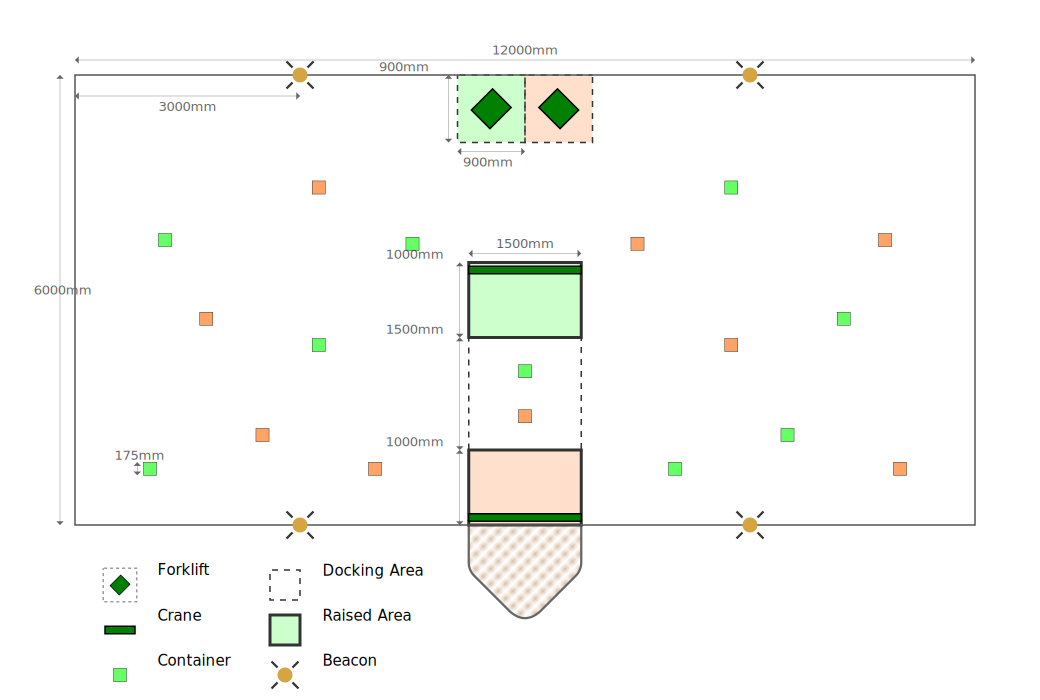
\includegraphics[scale=0.58]{fig-arena.pdf}
  \caption{Layout zones and tokens in the arena.}
  \label{fig:arena}
\end{figure}

\subsection{Containers}
\refstepcounter{SpecID}
\label{spec:containers}

\begin{enumerate}
  \item Containers are cuboids with side length \SI{260}{mm}.
  \item Containers are arranged as indicated in Figure~\ref{fig:arena}.
\end{enumerate}

\subsection{Forklift}
\refstepcounter{SpecID}
\label{spec:forklift}

\begin{enumerate}
  \item The forklift's footprint is a square with sides of length \SI{350}{mm}.
  \item TODO: Fetch the forklift dimensions from the simulator.
  \item The forklift is equipped with the following sensors:
  \begin{enumerate}
    \item Magnetic compass.
    \item Gyroscope.
    \item Accelerometer.
    \item Radio direction finder.
    \item Bump sensor.
    \item Ultrasonic distance sensor.
  \end{enumerate}
  \item The forklift is equipped with the following actuators:
  \begin{enumerate}
    \item Tank-steered driving wheels.
    \item Front grabber.
  \end{enumerate}
\end{enumerate}

\subsection{Crane}
\refstepcounter{SpecID}
\label{spec:crane}

\begin{enumerate}
  \item The crane is the full width of the ship, and \SI{100}{mm}
        in both other dimensions.
  \item The crane is equipped with the following sensors:
  \begin{enumerate}
    \item Accelerometer.
    \item Radio direction finder.
    \item Bump sensor.
    \item Ultrasonic distance sensor (mounted vertically).
  \end{enumerate}
  \item The crane is equipped with the following actuators:
  \begin{enumerate}
    \item Two-axis linear driving motor.
    \item Lifter.
  \end{enumerate}
\end{enumerate}
